%\documentclass{book}
\documentclass{article}                            %for shorter notes
\usepackage{graphicx}                              %for PNG images (pdflatex)
%\usepackage{graphics}                              %for EPS images (latex)
\usepackage[linkbordercolor={1.0 1.0 0.0}]{hyperref} %for \url tag
\usepackage{color}                                 %for defining custom colors
\usepackage{framed}                                %for shaded and framed paragraphs
\usepackage{textcomp}                              %for various symbols, e.g. Registered Mark
\usepackage{geometry}                              %for defining page size
\usepackage{longtable}                             %for breaking tables
%
\geometry{verbose,a4paper,tmargin=2.5cm,bmargin=2.5cm,lmargin=2.5cm,rmargin=2cm}
\hypersetup{
  pdfauthor = {Author Name},
  pdftitle = {Paper title},
  pdfsubject = {Paper subject},
  pdfkeywords = {Paper,keyword,comma-separated},
  pdfcreator = {PDFLaTeX with hyperref package},
  pdfproducer = {PDFLaTeX}
}
%
\bibliographystyle{IEEEtran}                       %a nice bibliography style
%
\def\efill{\hfill\nopagebreak}%
\hyphenation{Nordu-Grid}
\setlength{\parindent}{0cm}
\setlength{\FrameRule}{1pt}
\setlength{\FrameSep}{8pt}
\addtolength{\parskip}{5pt}
\renewcommand{\thefootnote}{\fnsymbol{footnote}}
\renewcommand{\arraystretch}{1.3}
\newcommand{\dothis}{\colorbox{shadecolor}}
\newcommand{\globus}{Globus Toolkit\textsuperscript{\textregistered}~2~}
\newcommand{\GT}{Globus Toolkit\textsuperscript{\textregistered}}
\newcommand{\ngdl}{\url{http://ftp.nordugrid.org/download}~}
\definecolor{shadecolor}{rgb}{1,1,0.6}
\definecolor{salmon}{rgb}{1,0.9,1}
\definecolor{bordeaux}{rgb}{0.75,0.,0.}
\definecolor{cyan}{rgb}{0,1,1}
%
%----- DON'T CHANGE HEADER MATTER
\begin{document}
\def\today{\number\day/\number\month/\number\year}

\begin{titlepage}

\begin{tabular}{rl}
\resizebox*{3cm}{!}{
\includegraphics{ng-logo.png}}
&\parbox[b]{2cm}{\textbf \it {\hspace*{-1.5cm}NORDUGRID\vspace*{0.5cm}}}
\end{tabular}

\hrulefill

%-------- Change this to NORDUGRID-TECH-NN

{\raggedleft NORDUGRID-TECH-NN\par}

{\raggedleft \today\par}

\vspace*{2cm}

%%%%---- The title ----
{\centering \textsc{\Large ARC accounting component}\Large \par}
\vspace*{0.5cm}
    
%%%%---- A subtitle, if necessary ----
{\centering \textit{\large Technical document}\large \par}
    
\vspace*{1.5cm}
%%%%---- A list of authors ----
    {\centering \large P\'eter D\'ob\'e \footnote{dobe@iit.bme.hu} \large \par}
    
%%%%---- An abstract - if style is article ----
%\begin{abstract}
%The abstract
%\end{abstract}
\end{titlepage}

%\tableofcontents                          %Comment if use article style
\newpage

\section{Purpose}

The ARC Usage Reporter tool is a component implementing accounting
functionality in the ARC middleware. Its objective is to gather
metered resource usage data for each job and submit it to an
accounting service along with the job submitter's identity and
miscellaneous job-related metadata. 

The accounting service stores the received usage data in a database,
and provides an interface for querying it.  Queries can be made by the
consumers of the accounting data, such as a billing component.  The
service itself is a third party application, separate from the
middleware distribution. The ARC Usage Reporter is currently capable
of using the logging service of the SweGrid Accounting System (SGAS),
but maintaining the possibility to enable utilizing other services
have been kept in mind during design.

Before the usage data collected from the resource manager is
submitted, it is transformed into records of job-level granularity. To
every job corresponds exactly one Grid user, therefore reports over a
time period (e.g.~an invoice) can be generated per-user, or
alternatively on a larger scale such as job project or VO level.

\section{Architecture}
  (diagram)

\begin{figure}[ht]
\centering{{\scalebox{0.9}{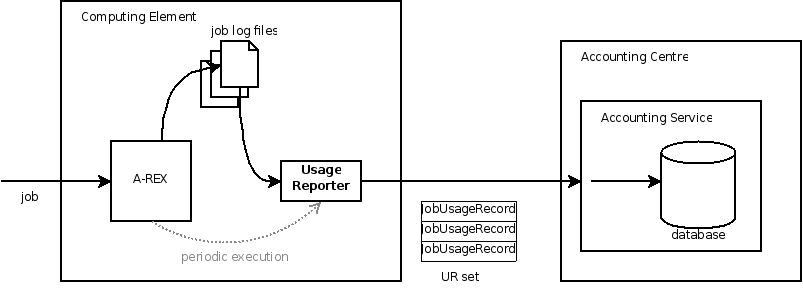
\includegraphics{usagereporting.png}}}
\caption{\label{fig:myfigure1}Components participating in accounting.} }
\end{figure}


  A-REX
  logger
  SGAS service

\section{Operation}

  \subsection{Invocation}
    stand-alone exe
    run by A-REX hourly
    command line arguments
    no config, everything from A-REX

  \subsection{Parsing job log files}
    ``id.randomletters''
    UR generated from them

  \subsection{Accessing LUTS}
    insert method
    certificates from:...

\section{Implementation}
  c++
  sw dependencies
    full arc
  install location

\appendix

\section{Configuration}
  jobreport
  jobreport\_options
  jobreport\_credentials

\section{Usage Record properties}
  input file format
  filled properties
  missing properties

\bibliography{grid}
\end{document}
